\subsection {Fundamentos matemáticos}
Para el desarrollo del presente proyecto se usará fuertemente la estadística, se observará la cantidad de veces que aparece la palabra clave en la base de datos recolectada para comprender el comportamiento o distribución que tiene. Además se buscará la relación que existe de la palabra clave con algún otro conjunto de palabras.\\

\noindent Para fundamentar todo el trabajo es importante definir algunos conceptos primordiales de la estadística.  Una  \emph{variable aleatoria} (v.a.) es la función real $X: \Omega\mapsto\mathbb{R}$ tal que el conjunto $\{\omega\in\Omega:X(\omega)\in I\}$ es un evento del espacio muestral $\Omega$ para cada intervalo $I\subset\mathbb{R}$. Existen dos tipos de variable, la primera de ellas es la \emph{variable aleatoria discreta} (v.a.d.), la cual está definida  cuando su rango de valores $R_x$ es finito o contablemente infinito y la segunda es la \emph{variable aleatoria continua} (v.a.c.), es aquella que puede tomar cualquier valor real en un intervalo.\\

%Una \emph{variable aleatoria} es una función asignando un número real $\mathbb{R}$ a cada posible resultado de un experimento. Con una muestra en espacio $S$, una variable aleatoria $X$ asigna el valor numérico $X(s)$ a cada resultado posible $s$ del experimento. La aleatoriedad viene del hecho que tenemos un experimento aleatorio (con probabilidades descritas por la función de probabilidad $P$). Las variables aleatorias simplifican la notación y expanden la habilidad de cuantificar y resumir resultados de experimentos.

%Se dice que una variable $X$ es discreta cuando si hay una lista finita de valores $a_,a_2,\ldots,a_n$ o un una lista infinita de valores $a_,a_2,\ldots$ de tal forma que $P(X=a_j$ para algún $j)=1$. Si $X$ es una variable aleatoria discreta, entonces el conjunto infinito o contable de valores $x$ tal que $P(X=x)$ se llama \emph{soporte} de $X$. En contraste una variable aleatoria continua puede tomar cualquier valor real en un intervalo.

%\subsubsection{Variable aleatoria comtinua)}
%A diferencia de las variables discretas, las \emph{variables aleatorias continuas} pueden tomar cualquier valor real en un intervalo y tienen una \emph{distribución continua}. Para obtener la probabilidad deseadaWHOMST, se debe integrar la función de densidad de probabilidad sobre el rango apropiado
%\begin{equation}
%P(X\in A)=\int_{A}f(x)dx
%\end{equation}
%\begin{displayquote}	``La forma más natural de expresar la distribución de v.a.d.s es la \emph{función de probabilidad}'' (\citeauthor{blitz19}, \citeyear{blitz19})\end{displayquote}

\noindent La \emph{distribución de probabilidad} es un modelo teórico que describe la forma en que varían o cambian los resultados de un experimento aleatorio, en otras palabras, a través de una función obtenemos las probabilidades de todos los posibles resultados que podrían obtenerse cuando se realiza un experimento aleatorio. Se hace una diferencia en las funciones de distribución para las variables aleatorias discretas y las variables aleatorias continuas.\\

\noindent Para  una v.a.d. $X$ con $\Omega=\{x_1,x_2, x_3,\ldots,x_n,\ldots\}$ donde $f(x)$ es la función de distribución, la probabilidad se encuentra dada por:
\begin{equation}
P(X=x)=\begin{cases}
0, & x\notin\Omega\\
f(x), & x\in\Omega.
\end{cases}
\label{eq:FP}
\end{equation}

\noindent Para  una v.a.c. $X$,  la función de densidad probabilística es una  función no negativa real $f:\mathbb{R}\mapsto[0,\infty)$, la probabilidad se encuentra dada por:
\begin{equation}
	P(X\in A)=\int_{A}f(x)dx.
\end{equation}
%El teorema de \emph{funciones de probabilidad válidas} dice que cuando $X$ es una variable aleatoria con soporte $x1,x2,\ldots$, la función de probabilidad $p_X$ de $x$ debe satisfacer los siguiente criterios:
%\begin{itemize}
%	\item No negativo $p_X (x) > 0$ si $x=x_j$ para un $j$, y $p_X(x)=0$, de otra forma;
%	\item Suma 1: $\sum_{j=1}^{\infty}p_X(x_j)=1$.
%\end{itemize}
%el primer criterio es verdadero porque la probabilidad es no negativa, el segundo es verdadero ya que $X$ debe tomar \emph{algún} valor, y los eventos ${X=xj}$ están disjuntos, entonces
%\begin{equation}
%\sum_{j=1}^{\infty}P(X=x_j)=P\bigg(\bigcup_{j=1}^{\infty}\{X=x_j\}\bigg)=P(X=x_1\ \text{ó}\ X=x_2\ \text{ó}\ \ldots)=1.
%\end{equation}
%Mientras que las distribuciones anteriores nos han dado toda la información acerca de la probabilidad de las variables aleatorias, cuando sólo se requiere un número que extraiga su valor, podemos utilizar la \emph{media}, también conocida como \emph{valor esperado}. Dada una lista de números $x_1,x_2.\ldots,x_n$, para obtener la \emph{media aritmética}, estos se suman y dividen entre $n$:
%\begin{equation}
%\bar{x}=\frac{1}{n}\sum_{j=1}^{n}x_j,
%\end{equation}
%la \emph{media ponderada} de $x_1,x_2.\ldots,x_n$ se obtiene de la siguiente forma:
%\begin{equation}
%\text{media ponderada}(x)=\frac{1}{n}\sum_{j=1}^{n}x_jP_j,
%\end{equation}
%donde los pesos $p_1,p_2.\ldots,p_n$ son números no negativos previamente especificados que suman a $1$.
%\subsubsection {Función de distribución acumulada}
%Esta función describe la distribución de todas las variables aleatorias (a diferencia de la función de probabilidad que sólo se aplica a las discretas). La \emph{función de distribución acumulada} de una variable aleatoria $X$ es la función $F_X$ dada por $F_X(x)=P(X\leq x)$ y tiene las siguientes propiedades:
%\begin{itemize}
%	\item Incrementos: Si $x_1\leq x_2$, then $F(x_1)\leq F(x_2)$.
%	\item Continua por la derecha: Es continua por la posibilidad de tener saltos. Cuando hay saltos es continua por la derecha, es decir, por cada $a$ se tiene
%	\begin{equation}
%	F(a)=\lim_{c\to a^+}F(x).
%	\end{equation}
%	\item Convergencia de $0$ y $1$ en los límites
%	\begin{equation}
%	\lim_{x\to \infty}F(x)=0\ \ \text{y}\ \lim_{x\to \infty}F(x)=1.
%	\end{equation}
%\end{itemize}
El \emph{valor esperado} o \emph{esperanza} de una v.a. $X$ discreta o continua, con una función de probabilidad $f(x)$  discreta o continua se define como
\begin{equation}
	\mu=E(X)=\sum_{x\in \Omega}xf(x),
	\quad
	\mu=E(X)=\int_{-\infty}^{\infty}xf(x)dx,
\end{equation}
respectivamente, la definición anterior  es también llamada la \emph{media} de $X$, cuyo uso es  similar a la media aritmética en estadísticas.\\


%si el soporte es finito, entonces se reemplaza por una suma finita, escribiéndose de la siguiente forma:
%\begin{equation}
%E(X)=\sum_{x}\underbrace{x}_\text{valor}\underbrace{P(X=x)}_{\begin{matrix}^\text{Función de}\\^\text{probabilidad}\\^\text{en $x$}\end{matrix}}.
%\end{equation}
%El valor esperado de una suma de variables aleatorias es la suma de sus valores esperados individuales, este es el teorema de la \emph{linealidad del valor esperado}, %donde para cada variable aleatoria $X,Y$ y cada constante $c$,
%\begin{equation}
%\begin{matrix}
%E(X+Y)=E(X)+E(Y),\\
%E(cX)=cE(X).
%\end{matrix}
%\end{equation}

\noindent Otro valor numérico importante que se usa para conocer la variabilidad de la distribución de cualquier v.a es la  \emph{varianza},  se define como
\begin{equation}
	\sigma^2=Var(X)=E(X^2)-E(X)^2.
\end{equation}

\noindent En la figura \ref{FIG:DISTS} se muestran las distribuciones más comunes para variables aleatorias discretas y continuas [\cite{bala20}]. \\

\noindent Una vez identificado el comportamiento de la variable aleatoria es útil pensar en la relación que tiene con otros tipo de variables. Un modelo de regresión lineal simple consiste en generar una recta que permita explicar la relación \emph{lineal} que existe entre dos variables. La variable dependiente $Y$ y la variable predictora o independiente $X$ se relacionan como:

\begin{equation}
	Y=\beta_0+\beta_1 X+\varepsilon,
	\label{recta}
\end{equation}
donde $\beta_0$, $\beta_1$ son valores estimados y $\varepsilon$ el error aleatorio con distribución normal. La ecuación (\ref{recta}) es una aproximación de la verdadera relación entre $X$ y $Y$, en el cual para un valor dado de $X$ el modelo es capaz de predecir un cierto valor para $Y$. Un ejemplo del modelo se muestra en la figura \ref{FIG:regresion}.\\

\begin{figure}[H]\centering
		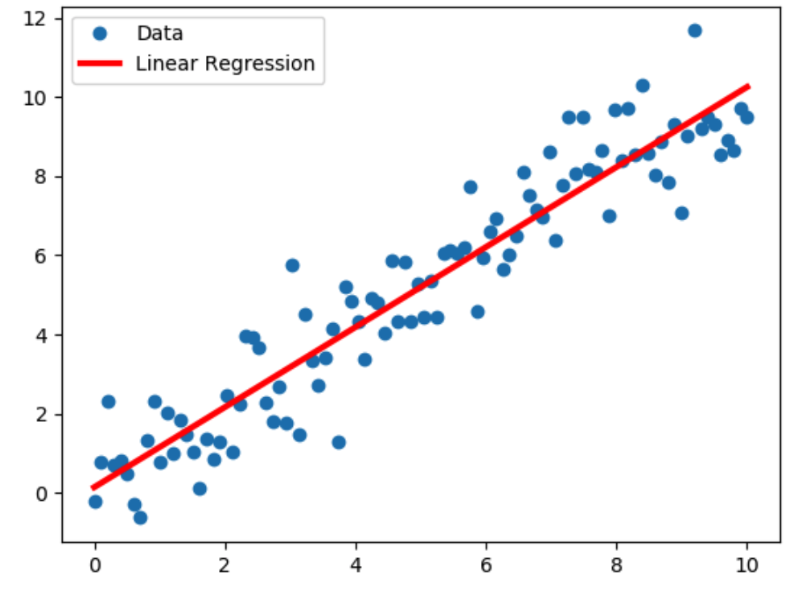
\includegraphics[scale=.3]{ej.png}
		\caption{Regresión lineal}\label{FIG:regresion}
	\end{figure}

\noindent La eficacia de la predicción del modelo lineal depende directamente de la estimaci\'on de los par\'ametros $\beta_0$ y $\beta_1$ para calcular la recta 
\begin{equation}
	\hat{y}=\hat{\beta}_0+\hat{\beta}_1x
\end{equation}
que se ajusta lo mejor posible a los datos con $E(\varepsilon)=0$.  Una vez determinadas las estimaciones puntuales de esos parámetros es conveniente calcular los intervalos de confianza para obtener una medida de precisión y más aún realizar contrastes de hipótesis para comprobar si un valor determinado puede ser el auténtico valor del parámetro.

Existe también otro modelo lineal donde relaciona la variable dependiente $Y$ con $K$ variables explícitas $X_1, X_2, \ldots, X_k$ de la forma:
\begin{equation}
	Y=\beta_0+\sum \beta_k X_k +\varepsilon
\end{equation}
donde $\varepsilon$ corresponde a los errores de los estimadores $\beta_k$.  Este modelo es llamado \emph{modelo lineal multivariable} y el procedimiento para los estimadores $\hat{\beta}_k$ sigue un procedimiento similiar al caso simple. \\

\noindent Una medida que será útil al relacionar dos variables será la  \emph{dependencia lineal} que exista entre ellas, se usará la \emph{covarianza}, la cual está definida como:
\begin{equation}
cov(X,Y)=E[(X-EX)(Y-EY)].
\end{equation}
Se sabe que si hay una relación lineal positiva, el valor de la covarianza será positiva y grande. En caso de que la relación lineal sea negativa, la covarianza será negativa y grande. Finalmente, cuando la covarianza es cercana a cero se sabe que no hay relación entre ambas variables.\\

La covarianza depende de las unidades de medida de las variables por lo que es conviente usar una medida que no dependa de las unidades, esta medida recibe el nombre de  \emph{coeficiente de correlación} definida como:
\begin{equation}
	r_{(X,Y)}=\frac{cov(X,Y)}{s_1s_2}
\end{equation}
donde $s_1$ y $s_2$ son las varianzas muestrales de las variables $X$ y $Y$ respectivamente.

En el caso del modelo lineal simple se busca que el valor de la pendiente de la recta  ($\beta_1$) sea distinto de cero, por lo que se pondrá un especial interés al contraste:
\begin{eqnarray}
	H_0: & \beta_1=0\\
	 H_1: & \beta_1\neq 0
\end{eqnarray}
donde la región de rechazo de la hipótesis nula es:
 
 \begin{equation}
\left|\frac{\hat{\beta_1}}{S/\sqrt{S{xx}}}\right| > t_{n-2,\alpha/2},
\end{equation}
donde $t_{n-2,\alpha/2}$ es la distribución de t-student con $n-2$ grados de libertad y un nivel de significancia de $\alpha$.

Utilizaremos el contraste de hipótesis para encontrar una mejor estimación de los parámetros $\beta_0$ y en particular $\beta_1$. Dicho procedimiento se puede consultar en [\cite{devo11}]



\begin{figure}[H]\centering\caption[Distribuciones]{Diversas distribuciones pueden modelar v.a.s, a continuación se muestran las mas importantes de acuerdo a \citeauthor{bala20} [\citeyear{bala20}].}\label{FIG:DISTS}$\begin{matrix}
\begin{subfigure}[t]{.3\textwidth}\includegraphics[width=1\linewidth]{binominal.png}\centering\\Binominal $b(n,p)$\end{subfigure}&
\begin{subfigure}[t]{.3\textwidth}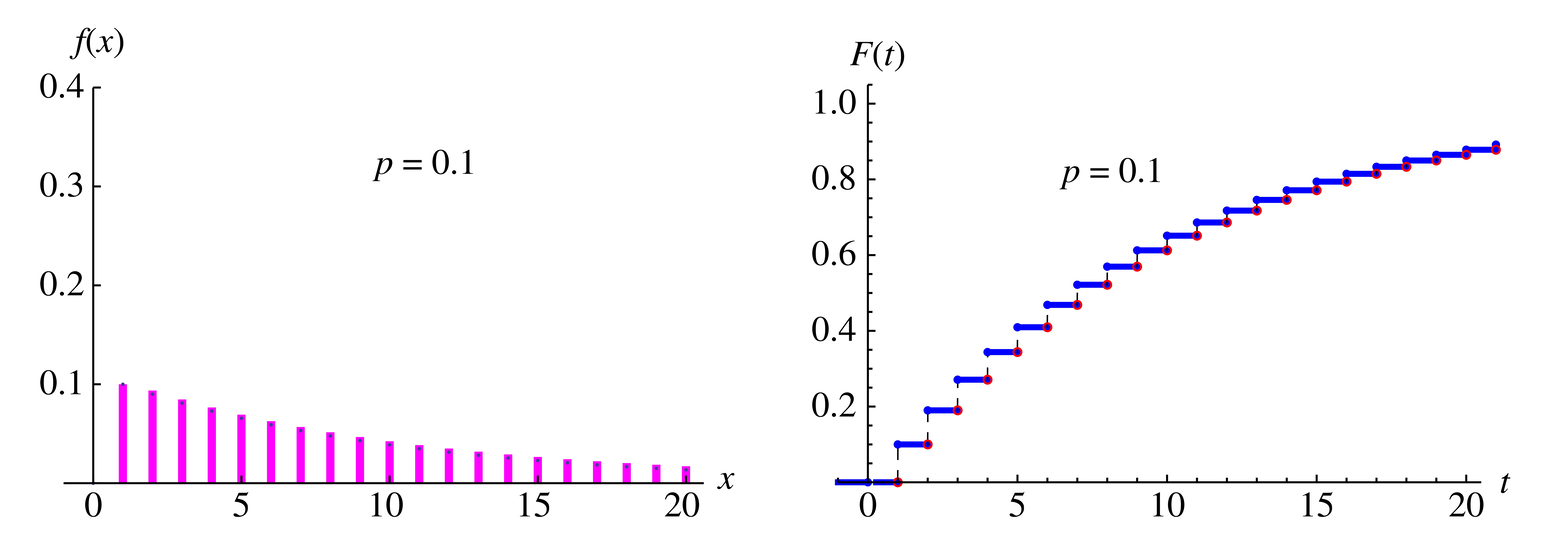
\includegraphics[width=1\linewidth]{geom.png}\centering\\Geométrica $G(p)$\end{subfigure}&
\begin{subfigure}[t]{.3\textwidth}\includegraphics[width=1\linewidth]{normal.png}\centering\\Normal $N(\mu,\sigma^2)$\end{subfigure}
\end{matrix}$\end{figure}
\begin{figure}[H]\centering$\begin{matrix}
\begin{subfigure}[t]{.3\textwidth}\includegraphics[width=1\linewidth]{epsilon_lambda.png}\\Exponencial $Expo(\lambda)$\end{subfigure}&
\begin{subfigure}[t]{.3\textwidth}\includegraphics[width=1\linewidth]{gama.png}\centering\\Gama $Ga(\alpha,\beta)$\end{subfigure}&
\begin{subfigure}[t]{.3\textwidth}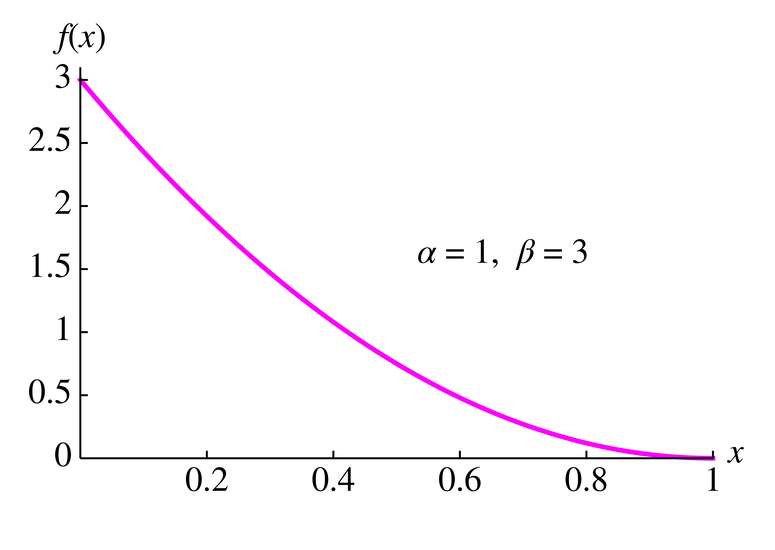
\includegraphics[width=1\linewidth]{beta.png}\centering\\Beta $Be(\alpha,\beta)$\end{subfigure}
\end{matrix}$\end{figure}


%Si $\alpha$ es la probabilidad deseada de cometer un error tipo I, la forma de la región de rechazo depende de la hipótesis alternativa. Las diversas alternativas de interés más frecuente y correspondientes regiones de rechazo son las siguientes:
%\begin{equation}  
%\begin{matrix}
%H_a\colon\rho>\rho0, &RR\colon z>z_\alpha\ \ \ \ \ \ \\
%H_a\colon\rho<\rho0, &RR\colon z<-z_\alpha\ \ \ \ \\
%H_a\colon\rho\neq\rho0, &RR\colon | z | >z_\alpha/2
%\end{matrix}
%\end{equation}

%La suma de los cuadrados del error \emph{SSE}, es es una alternativa para medie la variación en valores que permanecen sin explicación después de usar las $x$ para ajustar el modelo de regresión lineal simple, la razón $SSE/S_{yy}$ la proporción de la variación total en las $y_i$ que este modelo no explica. El coeficiente de determinación se puede escribir como
%\begin{equation}
%r^2=(\frac{S_{xy}}{\sqrt{S_{xx}S_{yy}}})^2=(\frac{S_{xy}}{S_{xx}})(\frac{S_{xy}}{S_{yy}})=(\frac{\hat{\beta_1}S_{xy}}{S_{yy}})=\frac{S_{yy}-SEE}{S_{yy}}=1-\frac{SSE}{S_{yy}}.
%\end{equation}

%Podemos interpretar a $r^2$ como la proporción de la variación total en las $y_i$  que es explicada por una variable $x$ en un modelo de regresión lineal simple.